\section{Depth First Search (DFS)}

\subsection{DFS Algorithms}

\begin{codebox}
    \Procname{$\proc{DFS}(s)$}
    \li $S = \proc{Stack}(\{ \, \})$ 
    \li $\proc{Push}(S,s)$ 
    \li \While $S \neq \emptyset$ \Do
        \li $u = \proc{Pop}(S)$
        \li \If $u$ is unvisited \Then
            \li visit $u$
            \li \For {\color{cyan} out} neighbor $v$ of $u$ \Do
                \li \If $v$ is unvisited \Then
                    \li $\proc{Push}(S,v)$   
\end{codebox}

An equivalent recursive version of the algorithm is presented in CLRS. $t$ is initialized to 0 prior to the first call to $\proc{DFS-Visit}$.

\begin{codebox}
    \Procname{$\proc{DFS-Visit}(s)$}
    \li visit $u$ 
    \li $t = t + 1$;\; $d[u] = t$ 
    \li \For {\color{cyan} out} neighbor $v$ of $u$ \Do
        \li \If $v$ is unvisited \Then
            \li $\proc{DFS-Visit}(v)$ 
            \End
        \End
    \li $t = t + 1$;\; $f[u] = t$
    \li $\proc{DFS-Vist}(s)$
\end{codebox}

The running time of the DFS algorithm is $O(m+n)$ if the graph is represented as an adjacency list, and $O(n^2)$ if represented as an adjacency matrix.

In DFS, we can keep track of the following two properties of each vertex:
\begin{itemize}
    \item $d[v]$: discovery time of vertex $v$ 
    \item $f[v]$: finish time of vertex $v$
\end{itemize}

\begin{theorem}
    In DFS of $G$, for all $u,v \in V$, either $(d[u],\, f[u])$ and $(d[v],\, f[v])$ are disjoint, or one is contained in the other. That is
    $$
    d[u] < f[u] < d[v] < f[v] \lor d[u] < d[v] < f[v] < f[u] \lor d[v] < d[u] < f[u] < f[v]
    $$
\end{theorem}

\begin{proof}
    Without loss of generality, suppose $d[u] < d[v]$. If $f[u] < d[v]$, then $d[u] < f[u] < d[v] < f[v]$. So suppose $d[v] < f[u]$, then $v$ is a descendant of $u$ if the DFS tree, so $\proc{DFS-Vist}(v)$ finishes before $\proc{DFS-Visit}(u)$, so $f[v] < f[u]$. Hence, $d[u] < d[v] < f[v] < f[u]$. The other case when $d[u] > d[v]$ is the mirror of this case.
\end{proof}

\subsection{Classification of Edges}

Tree edges: from $\pi(v)$ to $v$. $d[u] < d[v] < f[v] < f[u]$.

Back edges: from a node to an ancestor. $d[v] < d[u] < f[u] < f[v]$.

Forward edges: a non-tree edge from a node to a descedant. $d[u] < d[v] < f[v] < f[u]$.

Cross edges: between two nodes of which is a descendant of the other. $d[v] < f[v] < d[u] < f[u]$.

\begin{figure}[htbp]
    \centering
    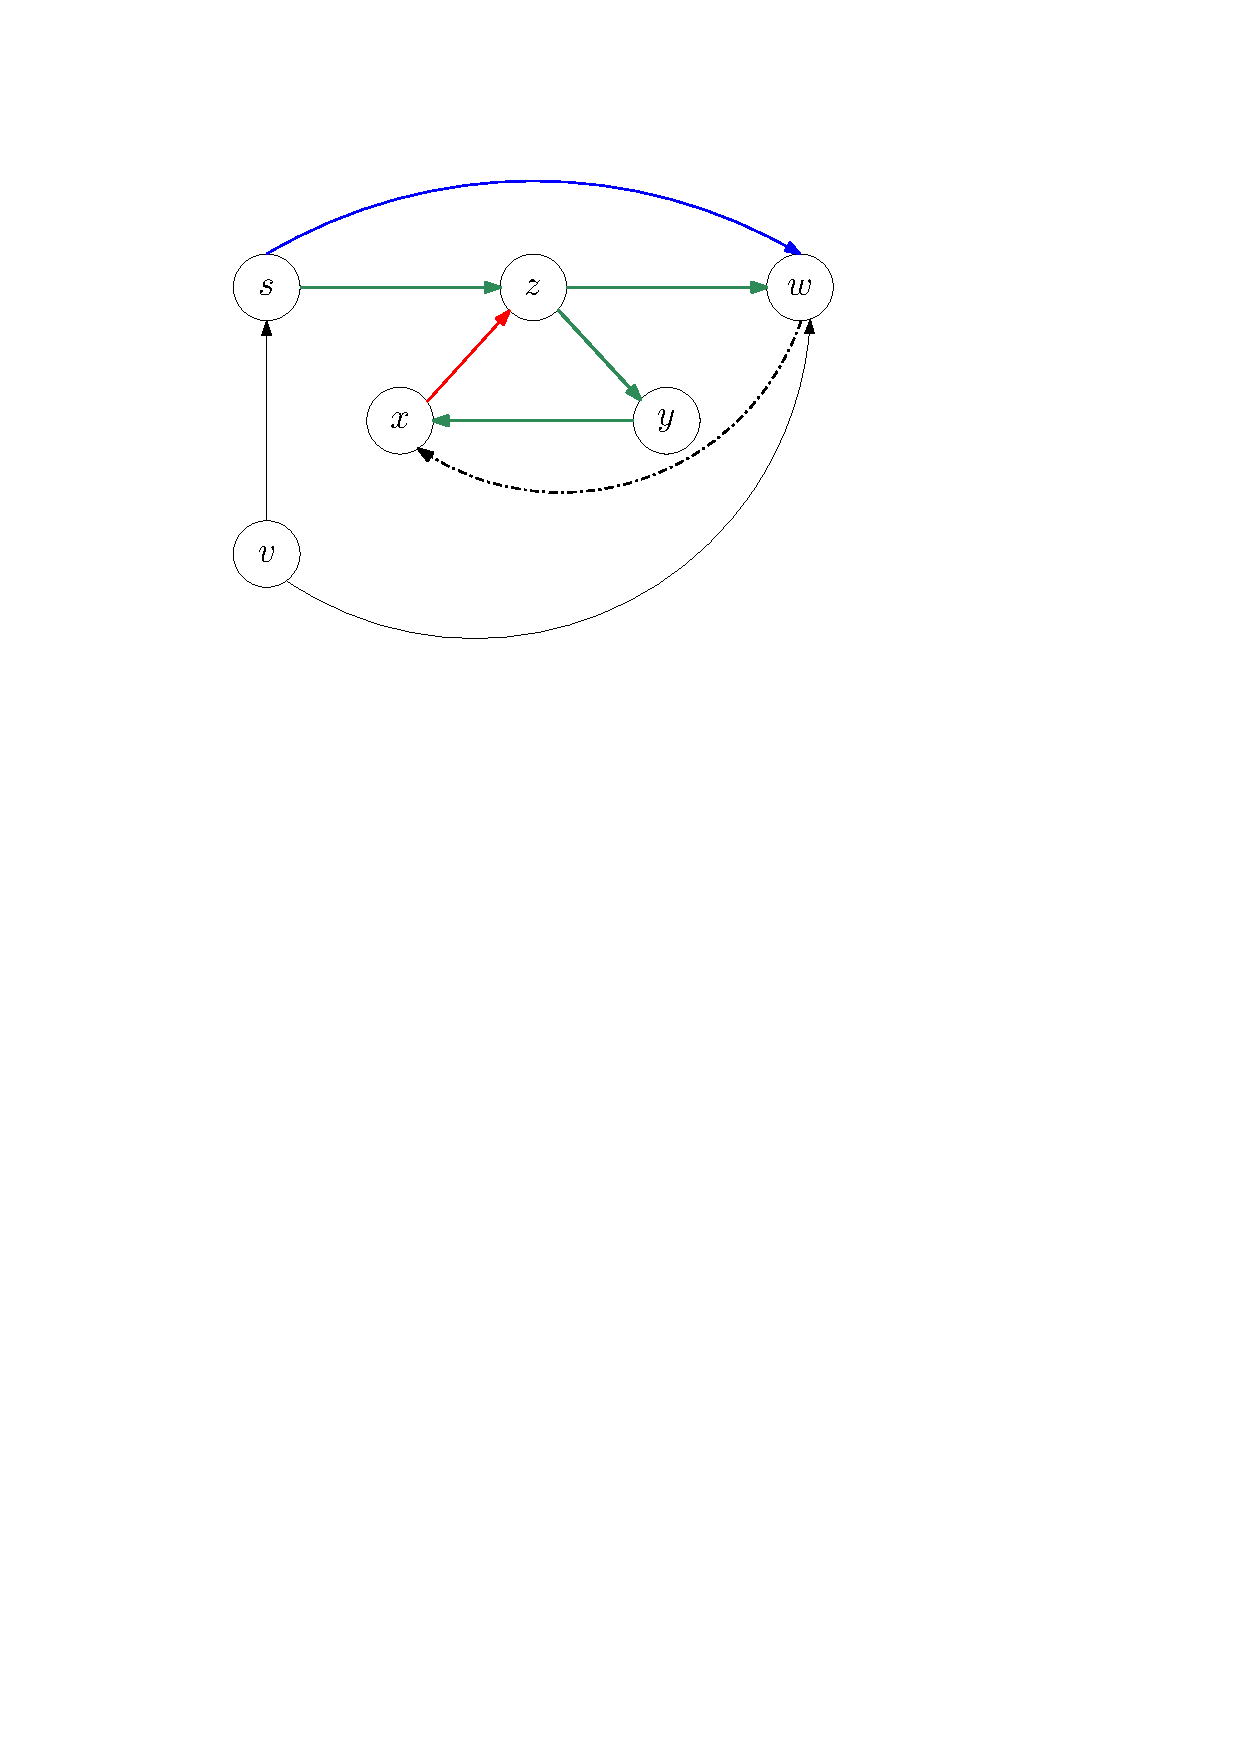
\includegraphics[width=0.4\linewidth]{dfs.pdf}

    \hfill

    \caption{Example of a DFS on a graph.}
    \label{fig:dfs-edges}
\end{figure}


\begin{theorem}
    In an undirected graph, all edges are either tree edges or back edges (we do not differentiate between forward edge and back edge because the graph is undirected).
\end{theorem}

\begin{proof}
    $\{u,v\} \in E$ and $d[u] < d[v]$. Since $v$ is visited before $\proc{DFS-Vist}(u)$ terminates, so $v$ is a descendant of $u$. So $\{u,v\}$ is a back edge or a tree edge.
\end{proof}

\section{Applications of BFS/DFS}

\begin{itemize}
    \item Broadcast information in a connected network.
    \item Detect if a graph contains a cycle. Every back edge is part of a cycle. If an undirected graph has no back edges. If all edges are tree edges, the graph is a tree and acylcic. 
\end{itemize}

\subsection{Cycle Detection}

\vspace{\parskip}

\begin{lemma}
    A directed graph is acyclic if and only if a DFS of the graph has no back edges.
\end{lemma}

\begin{proof}
    If there is a back edge, the graph has a cycle. Suppose the graph has a cycle. Before we finish the DFS of $u$, there is a predecessor $v$ of $u$ that is part of the cycle. $d[u] < d[v] < f[v] < f[u]$.
\end{proof}

\begin{lemma}
    An undirected graph contains a cycle if and only if its BFS tree contains a cross edge.
\end{lemma}

\subsection{Determining If a Graph is Bipartite}

\vspace{\parskip}

\begin{definition}
    A graph $G=(V,E)$ is a bipartite if and only if $V = A \cup B$ where $A,B \neq \emptyset$ and $A \cap B = \emptyset$ such that every edge $e \in E$ has 1 endpoint in $A$ and the other endpoint is in $B$. 
\end{definition}

Do BFS, record the parity of the distance of each node from the source.

\subsection{Topological Sort}

The topological sort of a directed acyclic graph (DAG) $G = (V,E)$. Ordering of the vertices of $V$ such that for if $(u,v) \in E$, then $u < v$. That is, $u$ is before $v$ in the ordering.

\begin{codebox}
    \Procname{$\proc{Topological-Sort}(G)$}
    \li $L = \{ \, \}$ 
    \li $\proc{DFS}(G)$ 
    \li \> after computing $f[v]$ for vertex $v$, insert $v$ at the front of $L$
    \li \Return $L$  
\end{codebox}

The algorithm sorts vertices in decreasing order of finish time.

\begin{theorem}
    \proc{Topological-Sort} is correct.
\end{theorem}

\begin{proof}
    Consider any edge $(u,v) \in E$, since $G$ is acyclic, it has no back edges.

    If $(u,v)$ is a tree edge or forward edge,
    $$
    d[u] < d[v] < f[v] < f[u]
    $$
    which is equivalent to $u < v$ in finish time.

    If $(u,v)$ is a cross edge.
    $$
    d[v] < f[v] < d[u] < f[u]
    $$
    $v$ is discovered and finished before the discovery and finish of $u$, so $u < v$ in finish time.
\end{proof}